\section[Sobre la convergencia de la aproximación]{Sobre la convergencia numérica de la exponencial imaginaria con dominio restringido.}

Para estudiar la velocidad de convergencia de la serie truncada \eqref{eq:iexpChebExpan} en el dominio $ x \in (-1, 1) $, primero es útil analizar 
individualmente cada uno de los factores de los términos de la sumatoria, principalmente los polinomios de Chebyshev y las
funciones de Bessel de primera especie.

Para los polinomios de Chebyshev se tiene que 
\begin{equation*}
	\abs{T_n(x)} \leq 1 \quad \forall x \in [-1, 1] \land n \geq 0,
\end{equation*}
de modo que no aportan nada concreto al estudio de la velocidad a la que converge la serie y se puede descartar.

Para las funciones de Bessel de primera especie, se tiene que para valores de orden $n$ enteros positivos mucho mayores
al argumento $z$, las funciones de Bessel se aproximan como
\begin{align*}
	J_n(z) &\sim \frac1{n!}\left( \frac{z}{2} \right)^n,\\
	\intertext{donde para gran $n$ el factorial se puede aproximar mediante la aproximación de Stirling $n! \sim \sqrt{2\pi n}\left( \frac{n}{e}\right)^n$}
	J_n(z) &\sim (2\pi n)^{-\frac12}\left( \frac{ez}{2n} \right)^n,
\end{align*}
la cuál converge rápidamente para $2n > ez$.

Debido a que la velocidad de convergencia está ligada al parámetro $z$, es útil analizar específicamente para qué casos
se aproximará la exponencial. Para la investigación corriente la exponencial se desea aproximar para el operador de
evolución temporal cuántico
\begin{equation}\label{eq:timeEvOp}
	\hat{U}(t) = \exp({\frac{i\hat{H}t}\hbar}),
\end{equation}
para aproximarlo (mediante polinomios de Chebyshev) en función del hamiltoniano, hace falta reescalarlo para que sus 
autovalores se encuentren entre -1 y 1, es decir
\begin{equation}\label{eq:reescaledHam}
	\tilde{H} = \frac{\hat{H} - \bar{E}}{\Delta E},
\end{equation}
donde $\bar E = \frac{E_\mathrm{max} + E_\mathrm{min}}2$ es el centro de banda y 
$\Delta E = \frac{E_\mathrm{max} - E_\mathrm{min}}2$ es el ancho de banda.

Sustituyendo el hamiltoniano reescalado \eqref{eq:reescaledHam} en el operador de evolución temporal \eqref{eq:timeEvOp}
\begin{align*}
	\hat{U}(t) &= \exp({\frac{i\Delta E\tilde{H}t}\hbar}) \exp(\frac{i\bar E t}\hbar) \\
	\hat{U}(t) &= \exp({\frac{i\tilde{H}t}\tau}) \exp(\frac{i\bar E t}\hbar)\\
	\hat{U}(t) &= \exp(i\tilde{H}\tilde t) \exp(\frac{i\bar E t}\hbar),
\end{align*}
donde $\tau = \frac\hbar{\Delta E}$ tiene unidades en el order de 
$\tau \sim \frac{0.6 \electronvolt\femto\second}{\electronvolt} = 0.6\femto\second$ 
por lo cuál la escala de $t$ está en el orden de los \femto\second. El fenómeno a estudiar 
(el tiempo de relajación en transporte eléctrico) está en el orden de los 
\femto\second{} a los \pico\second{} \autocite{Fan2018}, de modo que el cociente 
$\frac{t}{\tau} = \tilde{t} \in [10^0, 10^4)$.

\iffalse
\begin{figure}[bth]
	\centering
	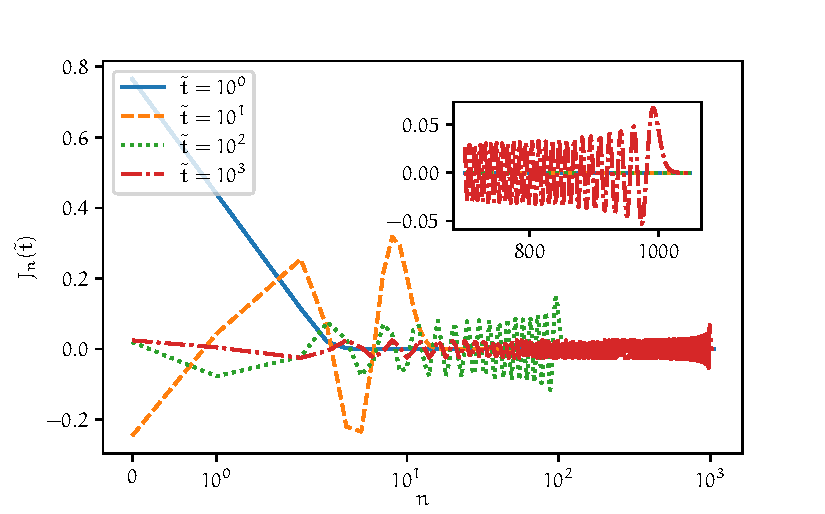
\includegraphics{./img/J_n(t).pdf}
	\caption{Gráficas de los polinomios de Chebyshev $J_n(t)$ para $N=1050$ términos. Se puede observar cómo los valores del polinomio decaen monotónicamente a partir de $n \approx t$ para cada valor de $t$.}
	\label{fig:gn_Jn(t)}
\end{figure}
\fi

\begin{figure}[htb]
	\centering
	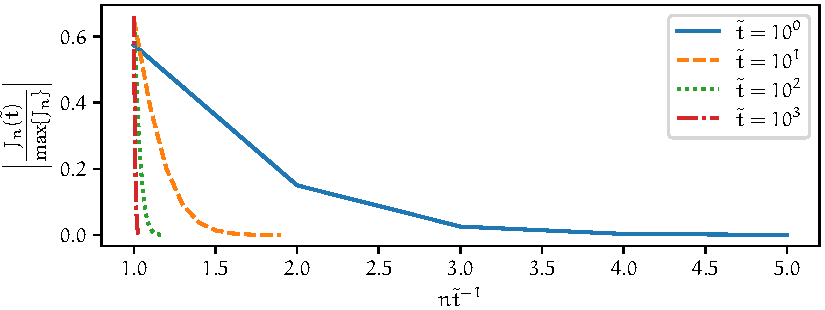
\includegraphics{./img/normJ_n(t).pdf}
	\caption[Funciones de Bessel Normalizadas]{Gráficas correspondientes al valor absoluto de las funciones de Bessel normalizadas en función de $n$ para valores menores de $1\times10^{-4}$; el eje $x$ se presenta escalado por el factor $\tilde{t}^{-1}$. Se puede ver como a partir de un término crítico $n_c$ las funciones de Bessel decaen pronunciadamente, donde $\frac n{\tilde t} \propto 1$, especialmente para valores altos de $\tilde{t}$.}
	\label{fig:normJ_n(t)}
\end{figure}

Todo esto implica que el argumento de las funciones de Bessel en la aproximación \eqref{eq:iexpChebExpan} está en el 
orden de $10^0$ a $10^3$. Para estos valores se tiene que la función de Bessel decae rápidamente para órdenes $N \propto 
z$ \autocite{Fan2018}, tal como se puede observar en la Fig.\ref{fig:normJ_n(t)}, de esta se puede concluir además que la
aproximación \eqref{eq:iexpChebExpan} se puede llevar a precisión arbitraria dependiente del número de términos a
utilizar.

\begin{figure}[htb]
	\centering
	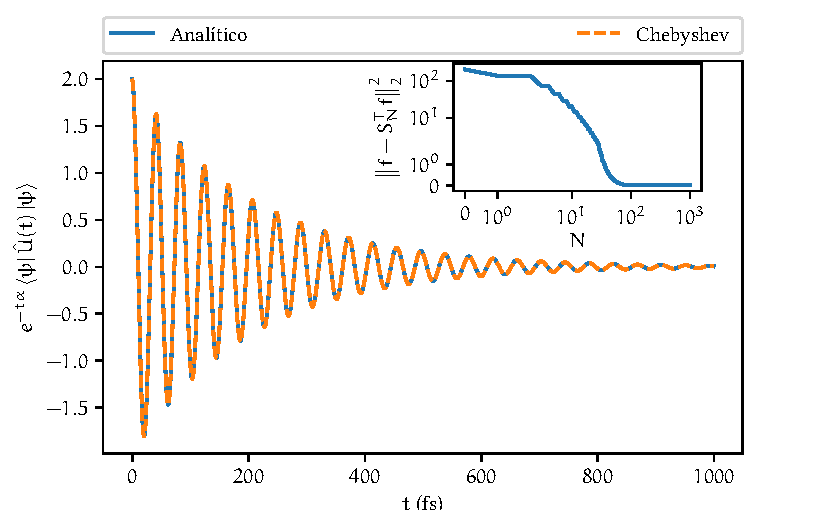
\includegraphics{./img/comparison.pdf}
	\caption[Valor esperado para el operador de evolución temporal amortiguado]{Comparación entre el cálculo analítico y la aproximación mediante polinomios de Chebyshev para el valor esperado amortiguado (por un factor $\alpha = 5\times 10^{-3}$) del operador de evolución temporal $\hat{U} = \exp(-i \hat{S}_z \tilde{t})$, $\hat{S}_z$ es la matriz de Pauli para el eje $z$ y $\tilde{t} = \frac{J_{\mathrm{ex}}t}{\hbar}$ donde $J_{\mathrm{ex}}\approxeq 100\milli\electronvolt$ es el acoplamiento de canje. La expresión analítica correspondiente al valor esperado es $2\cos{\tilde{t}}$. En el recuadro se muestra la norma Euclideana cuadrada de la diferencia entre la función correspondiente al cálculo analítico $f$ y su aproximación en serie de Chebyshev de orden $N$.}
	\label{fig:comparison}
\end{figure}

En la Fig.\ref{fig:comparison} se puede observar una demostración de la aproximación mediante los polinomios de Chebyshev para el valor esperado amortiguado del operador de evolución temporal. El amortiguamiento surge mediante el modelo de decoherencia cuántica, el cuál fue utilizado ya que otorga un enfoque más general a la demostración. En la gráfica se puede apreciar como la aproximación se sobrepone al valor analítico de la función, además de presentar que para órdenes de la aproximación mayores a $10^2$ la norma cuadrada de la diferencia entre la función analítica y la aproximación tiende drásticamente a $0$. 